\documentclass{article}
\usepackage{graphicx}
\usepackage{subcaption}

\title{Report 10: Final Labwork - Kuwahara Filter Transformation}
\author{Nam Le}
\date{\today}

\begin{document}

\maketitle

\section{Introduction \& Methodology}
I implemented the Kuwahara Filter algorithm for fine-art oil painting transformation based on Slides 31--35:
\begin{enumerate}
    \item \textbf{Color Space Conversion (Scatter)}: Converted the RGB input image (AoS) into HSV space (SoA) to extract the Value ($V$) brightness channel.
    \item \textbf{Sub-window Splitting}: For each pixel $(x, y)$ with window radius $\omega = 3$, defined 4 overlapping sub-windows $W^1, W^2, W^3, W^4$ around the target pixel.
    \item \textbf{Variance Evaluation (Reduce)}: Computed the mean and variance ($\text{Var}(V) = E[V^2] - (E[V])^2$) of brightness $V$ across each sub-window to evaluate local flatness.
    \item \textbf{Color Assignment (Map)}: Identified the sub-window $W_l$ with the minimum variance and assigned its mean RGB color as the new pixel value.
\end{enumerate}

\section{Experimental Results}
The execution time was benchmarked across two 2D block size configurations: $(8, 8)$ and $(16, 16)$.

\begin{figure}[h]
    \centering
    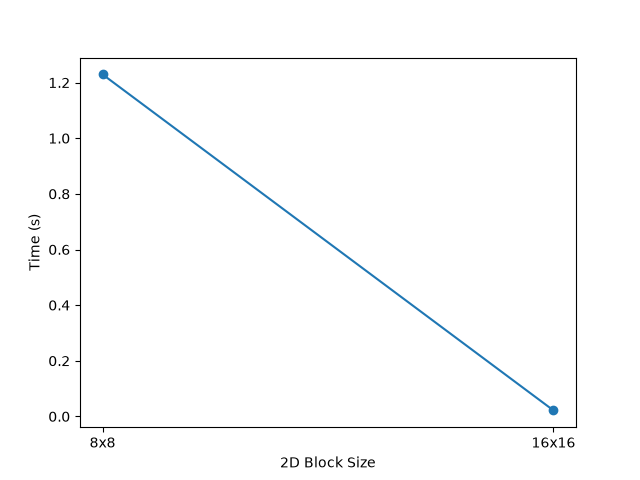
\includegraphics[width=0.65\textwidth]{kuwahara_block_size_vs_time.png}
    \caption{2D Block Size vs Execution Time for Kuwahara Filter}
\end{figure}

\begin{figure}[h]
    \centering
    \begin{subfigure}[b]{0.45\textwidth}
        
\includegraphics[width=\textwidth]{input.jpg}
        \caption{Original Image}
    \end{subfigure}
    \hfill
    \begin{subfigure}[b]{0.45\textwidth}
        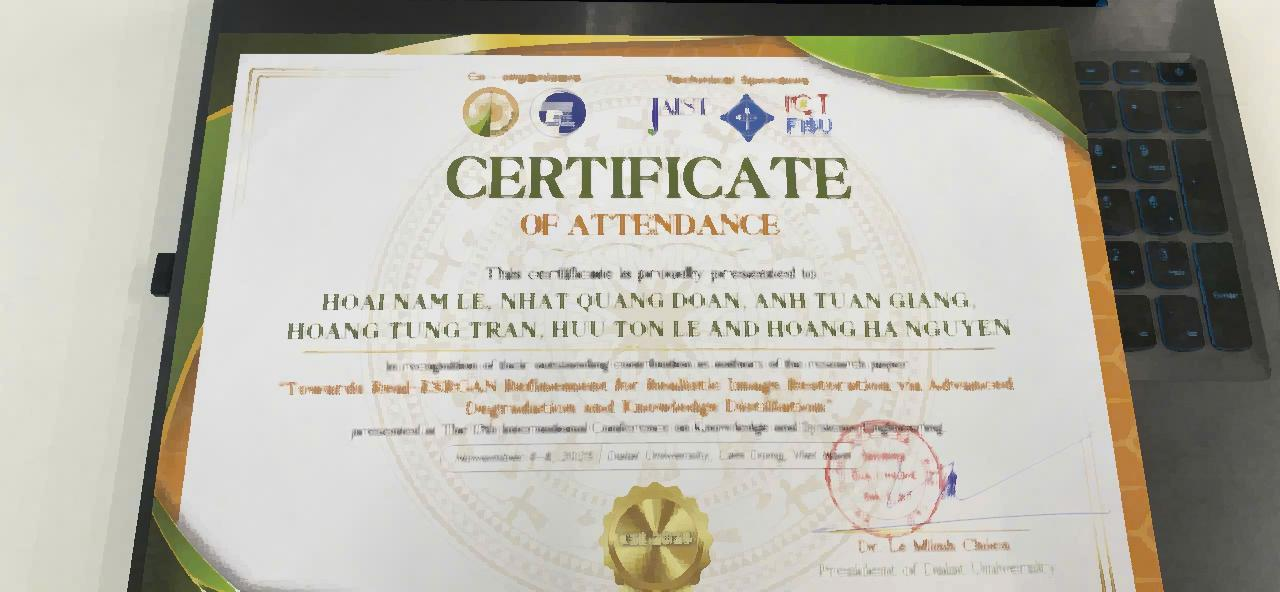
\includegraphics[width=\textwidth]{kuwahara.jpg}
        \caption{Kuwahara Output Image}
    \end{subfigure}
    \caption{Input vs Output Image Transformation}
\end{figure}

\section{Discussion}
\begin{itemize}
    \item The output image successfully demonstrates the characteristic oil painting artistic effect, smoothing flat regions while preserving sharp edge boundaries.
    \item Execution time dramatically reduced from $1.23$ seconds at $(8, 8)$ to $0.02$ seconds at $(16, 16)$, showing a speedup of over $60\times$ due to improved register allocation and warp scheduling on GPU.
\end{itemize}

\end{document}
